\documentclass[border=10pt]{standalone}
\usepackage{amsmath,amssymb,tikz-cd}
\definecolor{curveblue}{RGB}{30,80,180}
\definecolor{cusppurple}{RGB}{150,45,145}
\newcommand{\triangleframe}{%
  \path[use as bounding box] (-.85,-1.4) rectangle (4.85,4.8);
  \draw[gray!60,densely dashed] (0,0)--(4,0)--(2,3.464101615)--cycle;
}
\begin{document}
\begin{tikzcd}[column sep=4.5em]
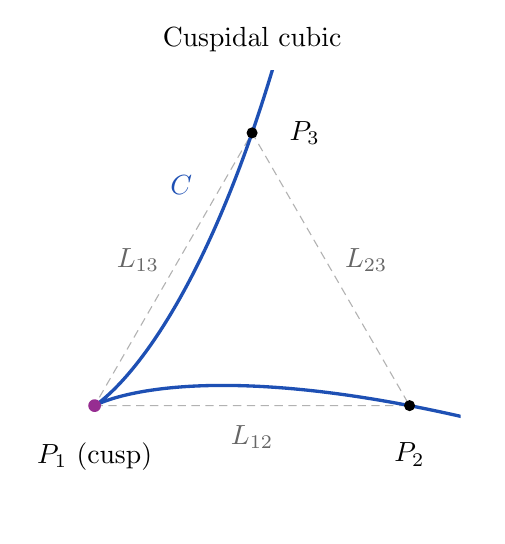
\begin{tikzpicture}[baseline=(current bounding box.center)]
  \triangleframe
  \begin{scope}
    \clip (-.65,-1.2) rectangle (4.65,4.25);
    % C: u(v-w)^2=4vw(v+w), with u+v+w=1.
    % Parametrization [u:v:w]=[1-t^2:(t^2+t^3)/2:(t^2-t^3)/2].
    \draw[curveblue,very thick,samples=350,domain=-1.3:1.3,variable=\t]
      plot ({3*\t*\t+\t*\t*\t},{sqrt(3)*(\t*\t-\t*\t*\t)});
  \end{scope}
  \fill[cusppurple] (0,0) circle (2.3pt);
  \node[below=10pt,align=center] at (0,0) {$P_1$\ (cusp)};
  \fill (4,0) circle (2pt) node[below=10pt] {$P_2$};
  \fill (2,3.464101615) circle (2pt) node[right=10pt] {$P_3$};
  \node[gray!80!black] at (2,-.4) {$L_{12}$};
  \node[gray!80!black] at (.55,1.85) {$L_{13}$};
  \node[gray!80!black] at (3.45,1.85) {$L_{23}$};
  \node[curveblue] at (1.1,2.8) {$C$};
  \node at (2,4.65) {Cuspidal cubic};
\end{tikzpicture}
\arrow[r,dashed,"\varphi"]
&
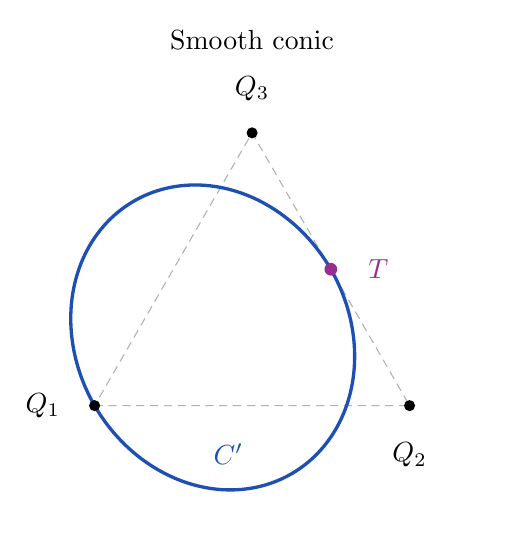
\begin{tikzpicture}[baseline=(current bounding box.center)]
  \triangleframe
  % The smooth conic (V-W)^2=4U(V+W).
  % Trigonometric parametrization covers its entire real affine locus.
  \draw[curveblue,very thick,samples=400,domain=0:180,variable=\t]
    plot ({3*cos(\t)^2-2*sin(\t)*cos(\t)},
          {sqrt(3)*cos(\t)^2+2*sqrt(3)*sin(\t)*cos(\t)});
  \fill (0,0) circle (2pt) node[left=9pt] {$Q_1$};
  \fill (4,0) circle (2pt) node[below=10pt] {$Q_2$};
  \fill (2,3.464101615) circle (2pt) node[above=8pt] {$Q_3$};
  \fill[cusppurple] (3,1.732050808) circle (2.3pt);
  \node[cusppurple,right=10pt] at (3,1.732050808) {$T$};
  \node[curveblue] at (1.7,-.62) {$C'$};
  \node at (2,4.65) {Smooth conic};
\end{tikzpicture}
\end{tikzcd}
\end{document}
